\section{Organizzazione SSN ed Economia aziendale}

\subsection{Organizzazione e legislazione sanitaria in Italia}

In una recente presentazione della legge di stabilità, è stato dichiarato un aumento del fondo sanitario nazionale per il 2017 a 113 miliardi.

Questo esempio è stato riportato perché, nella lezione di oggi, si tratterà di un argomento in cui la questione del fondo è fondamentale rispetto a tutto quello che il Servizio Sanitario può e deve fare.

\begin{itemize}
\item
  \textbf{Il sistema sanitario italiano è a base pubblica}: le cure più importanti vengono fornite dal sistema pubblico (SSN) a tutti, talvolta con dei ticket (ovvero co-pagamenti), sostenuto dalla tassazione generale.
Questo significa che non è che non paghiamo il SSN, ma che lo paghiamo con la tassazione generale: il fondo sanitario nazionale è cioè prelevato dal fondo generale di bilancio dello Stato, alimentato dalla
tassazione generale;
\item
  \textbf{I principi guida del SSN sono universalità, equità e solidarietà} (ex. L. 833/78): è uno dei pochi servizi sanitari ad essere retto da questi principi.
\end{itemize}

In Europa il servizio più simile al nostro è quello del Regno Unito, nel Nord America è quello canadese.

Nel Nord Europa esistono servizi misti (in parte pubblici, in parte sostenuti dalle casse previdenziali); mentre negli Stati Uniti il sistema è tutto privato per quel che riguarda le cure alla persona, così come lo è il sistema svizzero se si considera l'Europa.

Nei sistemi privati lo Stato spende comunque soldi, perché tutta la parte di sanità pubblica la deve spendere, ma non spende per la cura, l'ospedalizzazione, i farmaci e altro: perciò o i privati fanno fronte con i propri soldi oppure, come spesso succede nei sistemi, stipulano polizze assicurative in giovane età;

\begin{itemize}
\item
  \textbf{Sanità italiana ai primi posti nel mondo per le performance}:
  quando si mettono in rapporto nel mondo i costi per la sanità e le
  performance, ovvero i risultati in termini di salute, l'Italia è
  sempre in testa alle graduatorie;
\item
  \textbf{Indicatori sanitari tra i migliori del mondo:} il sistema
  sanitario italiano è uno dei sistemi più performanti al mondo:
  spendiamo relativamente poco e otteniamo molto.

Non è infatti un caso che la vita media, che è un importante indicatore
di salute, sia uno dei più alti al mondo;

\item
  \textbf{La sostenibilità attuale del SSN è precaria:} abbiamo un
  sistema pubblico, sta reggendo, ma in condizioni di grandissima
  precarietà;
\item
  \textbf{Volontà politica di mantenere il SSN pubblico.}
\end{itemize}

\subsubsection{I fattori di contesto}

\begin{itemize}
\item
  La \textbf{precarietà} prima citata è determinata dalla crisi: il SSN
  è alimentato dalla tassazione generale ed è noto che, quando c'è
  crisi, ci sono meno consumi meno introiti le casse sono più vuote;
\item
  \textbf{Longevità}: l'età media continua a salire;
\item
  \textbf{Migrazioni regionali per ricoveri}: alcune regioni attraggono
  i pazienti, perciò ci sono regioni da cui c'è migrazione sanitaria
  verso altre regioni, che hanno fama di avere strutture sanitarie
  pubbliche e private accreditate in grado di svolgere al meglio le
  funzioni di tipo ospedaliero-assistenziale;
\item
  \textbf{Differenze regionali}: ad esempio consideriamo la degenza
  pre-operatoria per interventi chirurgici elettivi, ovvero interventi
  che vanno a prenotazione del ricovero e dell'intervento a seconda
  della prescrizione del proprio medico o del medico specialista.
\end{itemize}

Quando si entra in ospedale per un intervento elettivo? Buona norma
sarebbe farlo il più tardi possibile, ovvero il più vicino possibile
all'intervento.

Bisogna infatti considerare che il costo di un giorno di degenza
ospedaliera è di 600 euro circa (costi di struttura, di personale, delle
tecnologie..).

Quindi il primo motivo per entrare il più tardi possibile è il poter
risparmiare giorni di degenza.

Il secondo motivo è rappresentato dalle infezioni ospedaliere e dai
batteri antibiotico-resistenti: più si sta in ospedale, maggiore è il
rischio di prenderseli.

In qualche caso si fanno anche interventi in day surgery, effettuabili
però solo in alcune condizioni (es. interventi di cataratta).

Quello che si deve cercare di fare è evitare i ricoveri per gli
interventi programmati, obiettivo che dovrebbe essere perseguito da
tutte le Regioni allo stesso modo, attraverso una buona organizzazione
(ad es. facendo gli esami pre-operatori in regime ambulatoriale, in modo
da completare la cartella pre-operatoria: in questo modo, anche se il
paziente si presenta la mattina stessa dell'intervento, può essere
operato nelle stesse condizioni di sicurezza in cui si troverebbe un pz
ricoverato a spese del SSN).

Se si facesse così, ci aspetteremmo di avere in giro per l'Italia
situazioni simili, ma così non è: alcune regioni hanno degenze medie
pre-operatorie per interventi chirurgici elettivi di circa 1 giorno (è
una media: una buona parte di pz entra il giorno stesso e conta 0, ma ci
sono altri pz che entrano 1 o più giorni prima per delle necessità
diagnostiche non gestibili in regime diverso), che è considerato un buon
indicatore.

La media nazionale è 1,38, ma è la distribuzione a destare perplessità:
ci sono Regioni importanti ,grandi e con tanti ricoveri, come il Lazio,
in cui si entra mediamente 2,24 giorni prima di un intervento elettivo
questo è indice di una carenza organizzativa, che ha un grande impatto
negativo sul bilancio regionale.

Si tratta di un esempio di inappropriatezza che dà un'idea di che cosa
oggi bisogna fare per sostenere il SSN: dare soldi in più, eliminare le
inappropriatezze e risparmiare dove si può.

\begin{itemize}
\item
  \textbf{La} \textbf{struttura del SSN} è costituita dal complesso
  delle funzioni, delle strutture, dei servizi e delle attività
  destinati alla promozione, al mantenimento e al recupero della salute
  fisica e psichica della popolazione senza distinzione di condizioni
  individuali o sociali (legge istitutiva del 1978).
\end{itemize}

Il SSN, preso nel suo complesso (strutture sanitarie, personale, volume
di fondi mosso..), è la più grande azienda d'Italia: muove, direttamente
e indirettamente, l'11\% del PIL.

Per effetto della legislazione vigente, i conti della sanità vengono
delegati alle Regioni: lo Stato stabilisce il fondo, il fondo viene
ripartito per abitanti alle Regioni e, nell'ambito regionale, la sanità
pesa per il 70-75\% del bilancio regionale.

Pertanto se la sanità va male, la Regione avrà i conti in passivo: i
deficit che così si sono formati sono stati pagati dallo Stato per un
certo periodo (facendo le leggi di fine anno), poi dal 2001 le Regioni
del Nord si sono opposte.

Da quel momento in avanti, le Regioni che non hanno saputo tenere il
bilancio sono state commissariate: sono stati nominati dei commissari
che cercano, nei limiti del possibile, di far rientrare le Regioni dai
disavanzi.

L'operazione di rientro dai disavanzi risulta però molto difficile: la
cultura organizzativa, infatti, non cambia da un giorno all'altro ed in
più, qualora ci fosse eccesso di personale, questo non può essere
licenziato.

Il concetto generale è quindi quello per cui, per poter garantire un
SSN, è necessario non solo remunerarlo adeguatamente, ma anche gestirlo
in modo appropriato facendo rientrare le Regioni in rosso.

\subsubsection{Prestazioni del SSN}

Le attuali prestazioni fornite dal SSN (gratuite o con compartecipazioni
di spesa/ticket -- LEA) ai cittadini italiani e a chi ne ha diritto ed è
sul nostro territorio nazionale sono:

\begin{itemize}
\item
  \textbf{Medico di famiglia}: attualmente i medici di medicina generale
  sono sotto pressione perché si è visto che dalle cattive prescrizioni
  e dall'iperprescrizione può dipendere il bilancio di una Regione.
\end{itemize}

La Regione Emilia-Romagna è stata la prima Regione a introdurre un controllo informatico di prescrizioni, ricette etc,: la Regione ha, per ciascun medico di famiglia, le cifre individuali spese per ciascuna delle voci di spesa sanitaria quando un medico è fuori dal range di normalità, viene chiamato a rendere conto del motivo e viene verificato se è un motivo giustificabile (es. medico di famiglia con numerosi assistiti portatori di una malattia cronica);

\begin{itemize}
\item
  \textbf{Pronto soccorso}
\item
  \textbf{Ricoveri ospedalieri acuti o lungodegenti}
\item
  \textbf{Prestazioni specialistiche ambulatoriali}
\item
  \textbf{Esami diagnostici e di laboratorio}
\item
  \textbf{Farmaci per malattie rilevanti (classe A)}
\item
  \textbf{Vaccinazioni}
\item
  \textbf{Screening oncologici e neonatali}
\end{itemize}

Su queste prestazioni le Regioni possono stabilire dei ticket, ovvero delle compartecipazioni di spesa. Che scopi ha il ticket?

\begin{itemize}
\item
  Contribuire in parte alla spesa;
\item
  Evitare gli sprechi (nell'anno in cui fu eliminato il ticket sui
  farmaci, il consumo dei farmaci aumentò del 30\% in 6 mesi quel 30\%
  altro non è stato se non cattiva prescrizione.
\end{itemize}

Perciò il ticket aveva ed ha, nel momento in cui è stato rimesso, lo scopo di calmierare i consumi laddove non necessari e ridurre le inappropriatezze.

E' stato inoltre messo un ticket al PS in base al codice di accesso: chi accede al PS con un codice bianco e poi va a casa, paga un ticket.

Addirittura alcune Regioni hanno stabilito che, a prescindere dal codice, se l'accesso al PS non dà ricovero bisogna pagare un ticket.

Si tratta di manovre per disincentivare l'uso improprio delle strutture sanitarie: c'è infatti la tendenza ad avere poca fiducia nella guardia medica e ad andare al PS ma se tutti ragionano così, le conseguenze sono:

\begin{itemize}
\item
  Pronti soccorsi affollati
\item
  Costi che aumentano
\item
  Inefficienza nelle prestazioni quando c'è realmente bisogno.
\end{itemize}

\subsubsection{Spesa Sanitaria in Italia}

Per quanto riguarda la spesa sanitaria pubblica in Italia, fino al 2008 c'è stato un incremento, poi la curva si è appiattita e, addirittura, nel 2013 c'è stato un decremento del fondo.

L'incremento verificatosi fino al 2008 è stato determinato da:

\begin{itemize}
\item
  Popolazione più anziana spese sanitarie maggiori;
\item
  Miglioramento delle tecnologie sistemi diagnostici e terapeutici più
  costosi.
\end{itemize}

Quindi sono stati il miglioramento tecnologico e il cambio demografico che hanno portato ad una situazione che era diventata insostenibile: quel tipo di crescita non era più compatibile con i bilanci dello Stato.

Per questo motivo sono cominciati i tagli, con cui il Governo ha sfoltito quelle che considerava spese superflue (in realtà, in molti casi, si sono fatti i cosiddetti ``tagli lineari'': si è tagliato in tutte le Regioni allo stesso modo per tutte le prestazioni il risultato è stato quello di risparmiare qualcosa ma, in alcuni casi, si è scesi sotto il livello per poter garantire una buona qualità delle cure).

La politica dei tagli lineari è molto criticata, ma è quella più semplice da fare.

L'ideale sarebbe tagliar effettivamente dove c'è il superfluo e lasciare le cose come stanno dove c'è efficienza.

In media il SSN spende 1882 euro all'anno per cittadino (6,8\% del PIL italiano): è una media, infatti la popolazione sana mediamente ha bisogno di poche cure, mentre se consideriamo la popolazione anziana con malati cronici allora i costi possono essere anche molto superiori.

I miliardi stanziati per la spesa sanitaria vengono ripartiti tra le Regioni in base al numero di residenti (l'iter è: approvazione legge di stabilità il Governo arriva alla conferenza Stato-Regioni ripartizione).

Il problema è che, in alcune Regioni, i pazienti non vanno nelle strutture ospedaliere della Regione, ma vanno a farsi curare fuori Regione: la conseguenza è che quelle Regioni hanno ospedali più vuoti e posti letto liberi di fatto però le Regioni da cui i pazienti migrano non risparmiano sui costi perché i costi fissi non vengono eliminati, mentre le Regioni in cui i pazienti migrano incassano la prestazione e riescono a lavorare ribilanciando.

Questo sta creando un grande problema, tant'è che adesso nella legge di stabilità è stato messo un freno alle migrazioni: si può sempre circolare, ma solo per interventi di alta specialità (non per gli altri interventi e nemmeno per i ricoveri ordinari).

In aggiunta a questo meccanismo bisogna anche considerare che quando la gente è in una zona in cui manca la fiducia nell'ospedale, tende ad andare o in un'altra Regione (come è stato detto) o nel privato: abbiamo infatti una quota di spese private derivate dalle prestazioni non date dal SSN (es. odontoiatria, a meno che non ci sia una malformazione o un incidente dove è necessario ricostruire i denti) e da ricoveri in strutture private.

\textbf{La ripartizione della spesa sanitaria in Italia} è la seguente:

\begin{itemize}
\item
  Pubblica 77,2\%
\item
  Out of pocket 18,7\% (=pagamento alla prestazione, ovvero ciò che non
  è compreso nei livelli essenziali di assistenza, e farmaci non di
  classe A, cioè i farmaci da banco)
\item
  Intermediata 4,1\% (fondi integrativi 77,3\%, polizze assicurative
  22,7\%).
\end{itemize}

Rappresentano spese private:

\begin{itemize}
\item Farmaci C
\item Ticket
\item Odonto
\item Omeopatia
\item Estetica
\item Extra LEA
\item Assicurazione
\item Fondi
\end{itemize}

Un altro esempio di differenza regionale è quella rappresentata
dall'alta tendenza che le donne hanno, in alcuni luoghi (es. Roma), ad andare a partorire in casa di cura, pagando out of pocket.

A cosa è dovuto questo?
\begin{itemize}
\item Sfiducia nella struttura pubblica;
\item Scarsa qualità e cattiva organizzazione della struttura pubblica.
\end{itemize}

Questi sono gli aspetti su cui lavorare, tant'è vero che c'è un dato emblematico preso dalle statistiche: nelle Regioni del Nord esistono strutture private e, quasi tutte, sono accreditate dal SSN (il Servizio Sanitario Regionale nel dare gli accreditamenti valuta se c'è o meno il bisogno).

Per quanto riguarda la nostra realtà, in Emilia-Romagna vengono dati pochi accreditamenti alle strutture private: la Regione, infatti, ritiene di avere una rete di strutture pubbliche sufficiente per poter coprire quasi tutte le necessità dei suoi cittadini.

E' quindi importante avere chiaro il concetto che il SSN, laddove non ha le sue strutture, si convenziona e si avvale anche delle strutture private accreditate.

Il fondo sanitario nazionale è così tripartito:

\begin{itemize}
\item
  Assistenza ospedaliera 46,97\%
\item
  Assistenza distrettuale 48,84\% (medico di famiglia, visite
  specialistiche, farmaci di classe A, esami di lab, esami diagnostici
  fuori dall'ospedale\ldots{})
\item
  Prevenzione 5\% (questa fetta deve essere interpretata come un
  investimento e, spesso, viene sacrificata).
\end{itemize}

\subsubsection{Livelli Essenziali Uniformi di Assistenza (LEA)}

Il SSN assicura ai cittadini di tutte le regioni i livelli essenziali e uniformi di assistenza (LEA), definiti nel rispetto dei principi della dignità della persona, del bisogno di salute, dell'equità nell'accesso, della qualità delle cure e della loro appropriatezza riguardo alle specifiche esigenze.

L'individuazione dei LEA è fatta dallo Stato che, però, deve avere la copertura finanziaria: il tutto perciò rientra nella Legge di bilancio.

E' talmente difficile aggiornare i LEA che non si è ancora riusciti a farlo, nonostante 15 anni di tentativi.

\textbf{Altre attività di prevenzione} (nei LEA, gratuite e inserite nel 5\% per la prevenzione) sono:

\begin{itemize}
\item
  Sorveglianza, prevenzione e controllo delle malattie infettive e
  parassitarie (inclusi i programmi vaccinali);
\item
  Tutela della salute e della sicurezza degli ambienti aperti e
  confinati;
\item
  Sorveglianza, prevenzione e tutela della salute e sicurezza nei luoghi
  di lavoro;
\item
  Salute animale e igiene urbana veterinaria;
\item
  Sicurezza alimentare -- Tutela della salute dei consumatori (es.
  vigilanza sulla catena alimentare, sulle bevande\ldots{});
\item
  Sorveglianza e prevenzione delle malattie croniche, inclusi la
  promozione di stili di vita sani ed i programmi organizzati di
  screening, sorveglianza e prevenzione nutrizionale (tutte attività
  gestite dalle ASL nell'ambito del 5\% dei fondi dedicati alla
  prevenzione);
\item
  Attività medico legali per finalità pubbliche.
\end{itemize}

\subsubsection{Struttura del SSN}

\textbf{Tre livelli:}

\begin{itemize}
\item
  \textbf{Centrale} -- Ministero della Salute e Organi tecnici;
\item
  \textbf{Regionale} (dal 2001 le Regioni hanno assunto più autonomia,
  soprattutto sul fronte organizzativo);
\item
  \textbf{Locale} -- Aziende USL e Aziende ospedaliere.
\end{itemize}

\paragraph{Organizzazione delle aziende sanitarie}

\begin{itemize}
\item Aziende USL (suddivisione territoriale)
\item Aziende Ospedaliere (identificati dalle Regioni)
\end{itemize}

\begin{figure}[!ht]
\centering
	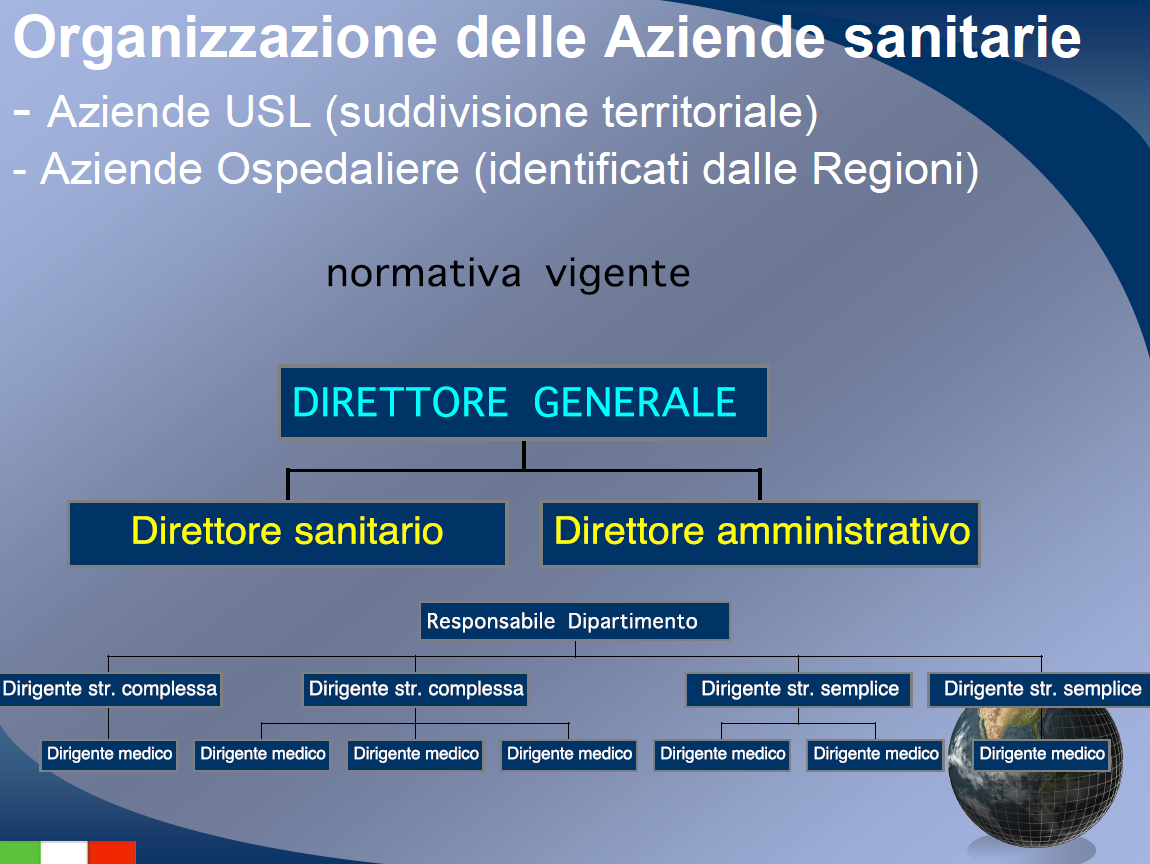
\includegraphics[width=0.7\textwidth]{13/image1.png}
	\end{figure}

Nell'ambito delle aziende sanitarie locali, a partire dagli anni '90 (dopo modifica della Legge sanitaria del 1978), è stata creata la figura di un manager: il \textbf{Direttore generale}, figura che cerca di gestire al meglio i fondi (ogni direttore generale gestisce circa 1 miliardo) e che ha un mandato della durata di 5 anni. Circa 1/3 degli attuali manager è medico chirurgo con la specialità in Igiene e Medicina preventiva, 1/3 è medico con altre specialità e 1/3 è di estrazione di vario tipo (prevalentemente giuridico-economica).

Se il manager non è un medico, è necessario che scelga poi con attenzione i suoi due collaboratori diretti: il \textbf{Direttore sanitario} (medico) e il \textbf{Direttore amministrativo} (contabile).

Ovviamente invece laddove c'è un Direttore generale medico, il Direttore sanitario è pur sempre importante, ma lo è meno rispetto a quando il Direttore generale è una figura giuridica che lascia in mano al suo collaboratore diretto dei temi specifici.

Il Direttore generale è nominato dalla Regione, mentre i Direttori sanitario e amministrativo sono nominati per nomina fiduciaria
direttamente dal Direttore generale (sono tutte figure che restano in carica 5 anni).

Tutta la struttura del SSN poi è retta dai \textbf{livelli dipartimentali}: tutti gli ospedali sono suddivisi in dipartimenti ciascun dipartimento ha un responsabile etc.

\subsubsection{Attualità: Referendum 04/12/16}

Cosa implica, per quanto riguarda la Sanità, la modifica costituzionale proposta e votata dal Parlamento e sottoposta al Referendum del 4 dicembre 2016?

\begin{itemize}
\item
  In questo momento la Sanità è gestita, in via concorrente, dallo Stato
  e dalle Regioni: lo Stato divide il fondo e detta i principi generali,
  le Regioni agiscono per fornire le prestazioni e organizzare al meglio
  i servizi. Pertanto spetta alle Regioni la potestà legislativa, salvo
  che per la determinazione dei principi fondamentali, che è riservata
  alla legislazione dello Stato.
\end{itemize}

Uno dei problemi che ci sono stati dal 2001 ad oggi è che si sono verificati circa 500 contenziosi tra Stato e Regioni: in alcuni casi perché lo Stato si è appellato alla Corte Costituzionale per leggi regionali ritenute in eccesso di potere, sovrapponendosi a norme statali, in altri casi sono invece state le Regioni a citare il Governo davanti alla Corte Costituzionale per aver ecceduto nei compiti (di solito quando c'è un conflitto Stato-Regione vince lo Stato: normalmente le connessioni e lo scambio di informazioni tra il Governo e la Corte Costituzionale, in termini di pareri su certi provvedimenti, sono maggiori di quello che succede a livello regionale);

\begin{itemize}
\item
  Con la norma sottoposta a Referendum si avrebbe l'abolizione della legislazione concorrente per tutte le materie, perché ritenuta un modo poco utile per procedere.
\end{itemize}

Pertanto per tutte le materie, che sono circa 15 (trasporti, ambiente, energia..), la norma o la dà lo Stato o la danno le Regioni.

La tendenza è quella di dare quasi tutto allo Stato, quindi la modifica costituzionale è centralista.

Per quanto riguarda la Sanità, questa è stata divisa in 2: lo Stato ha legislazione esclusiva in determinate materie (determinazione dei LEA, previdenza sociale, tutela e sicurezza del lavoro, politiche attive\ldots{}) con la norma si irrobustisce il potere statale in materia sanitaria.

Cosa resta alle Regioni? La potestà legislativa in programmazione e organizzazione dei servizi sanitari e sociali.

Quindi si darebbe praticamente tutto allo Stato, salvo programmazione e organizzazione dei servizi sanitari: lo Stato detterebbe le regole generali molto più di oggi, però tutta l'organizzazione e la programmazione verrebbe lasciata alle Regioni, che avrebbero più autonomia perché, a quel punto, sarebbero materie di loro piena competenza.
